%
% $Id: blank.tex,v 2.0 2010-01-05 18:50:50+09 kobayasi Exp $
%
% Mar 21, 2001:  Revision Control Started!!
%
\documentclass[11pt]{jarticle}
\usepackage{newcent}             % PDFへの変換後の品質を高める
\usepackage[dvipdfmx]{graphicx}
\usepackage{wrapfig} % 文章を図に回り込ませて配置するもの
\usepackage{comment} % 複数行をコメントアウトするためのもの
\usepackage{color}
\definecolor{purple}{rgb}{0.6,0,0.4}
\definecolor{brown}{cmyk}{0,0.81,1,0.60}
\usepackage{listings, jlisting}
\renewcommand{\lstlistingname}{ソース}
\lstset
{
language=Java,
numbers=left,
breaklines = true,
basicstyle={\small},
identifierstyle={\small},
keywordstyle={\small\bfseries\color{purple}},
commentstyle={\small\itshape\color{brown}},
stringstyle={\small\ttfamily},
frame=single,
tabsize=4
}
\usepackage{otf}

%
%\usepackage[doctor]{gaiyo}      % 博士論文要旨の場合
%\usepackage[master]{gaiyo}      % 修士論文要旨の場合
\usepackage{gaiyo}               % 卒業研究概要の場合
% \usepackage[junior]{gaiyo}      % 専門演習レポートの場合

\title{スマートフォンのモーションセンサを利用した個人認証アプリケーションの開発}
\id{情11-170}
\author{\UTF{9AD9}坂 賢佑}
\teacher{小林 孝史}

\begin{document}
\maketitle

\section{はじめに}
スマートフォンが徐々に普及しつつある現在,スマートフォンの個人認証方法は画面上に表示されるソフトウェアキーボードのテンキーを用いたパスコード認証が大部分を占めている.
しかし,この認証方法は画面ロックを解除するたびに画面に表示されたソフトウェアキーボードを目で見て指でタッチして操作する必要があるため,ユーザにとっては煩雑な作業である.
また,あらかじめ決められた文字種の中から一つずつ選択したものを元にパスコードを構築していくという性質上,パターン数が限られ自由度が限定されてしまう.

そこで,本研究ではパスコード認証が抱える認証の煩雑さを解消し,かつ自由度が高くより直感的に個人認証を行えるアプリケーションを開発する.
このアプリケーションには,一般的なスマートフォンに搭載されている加速度センサとジャイロセンサを用いる.

% 増幅-ローパス-ずらし
\section{本研究のシステム}
本研究では兎澤の研究\cite{tozawa}で挙げられていた全体的な認証成功率の低さ,特に手首を中心とするような比較的動きの小さいモーションに対する認証成功率の改善を目標とする.
システムの動作フローを図\ref{flow}に示す.

\begin{wrapfigure}{r}{80mm}
    \begin{center}
        %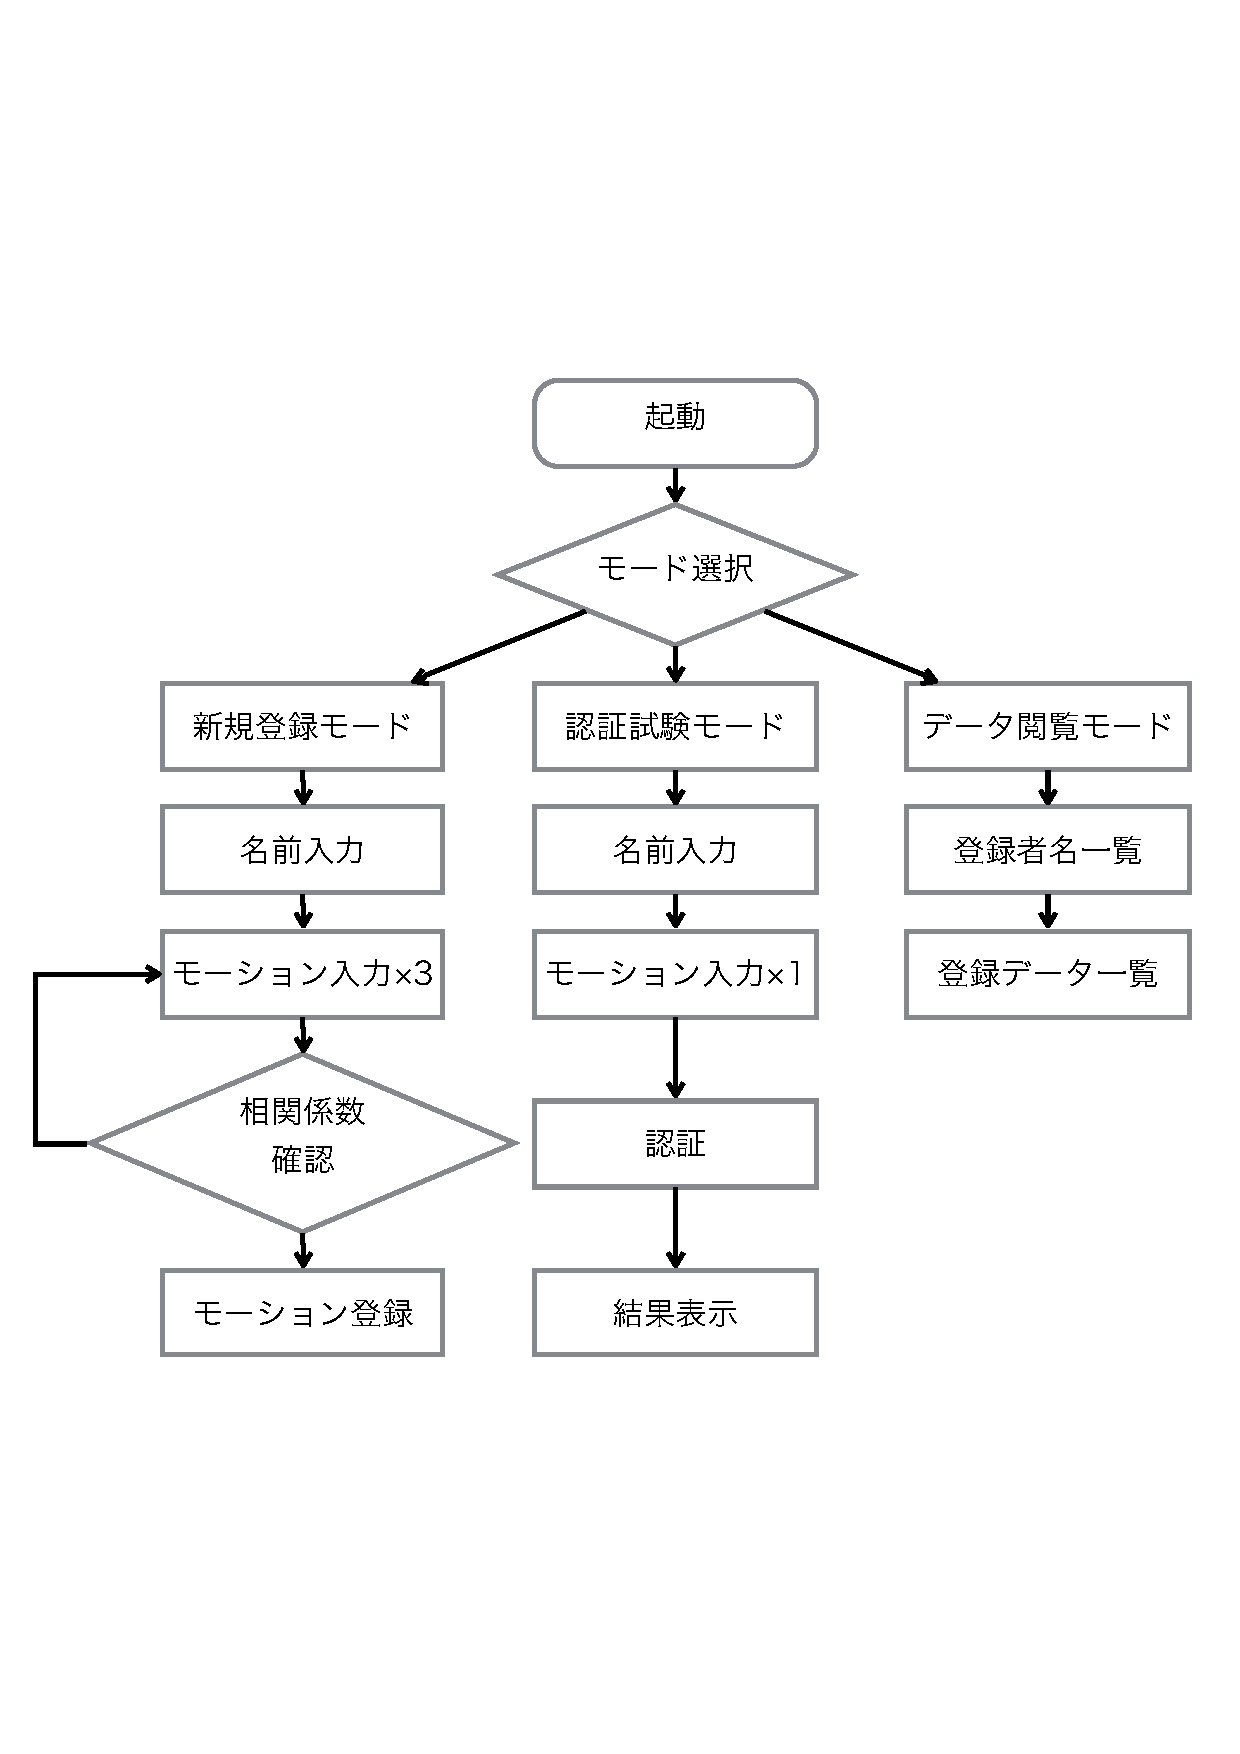
\includegraphics[width=70mm, bb=0 183 594 670]{Flow.pdf}
        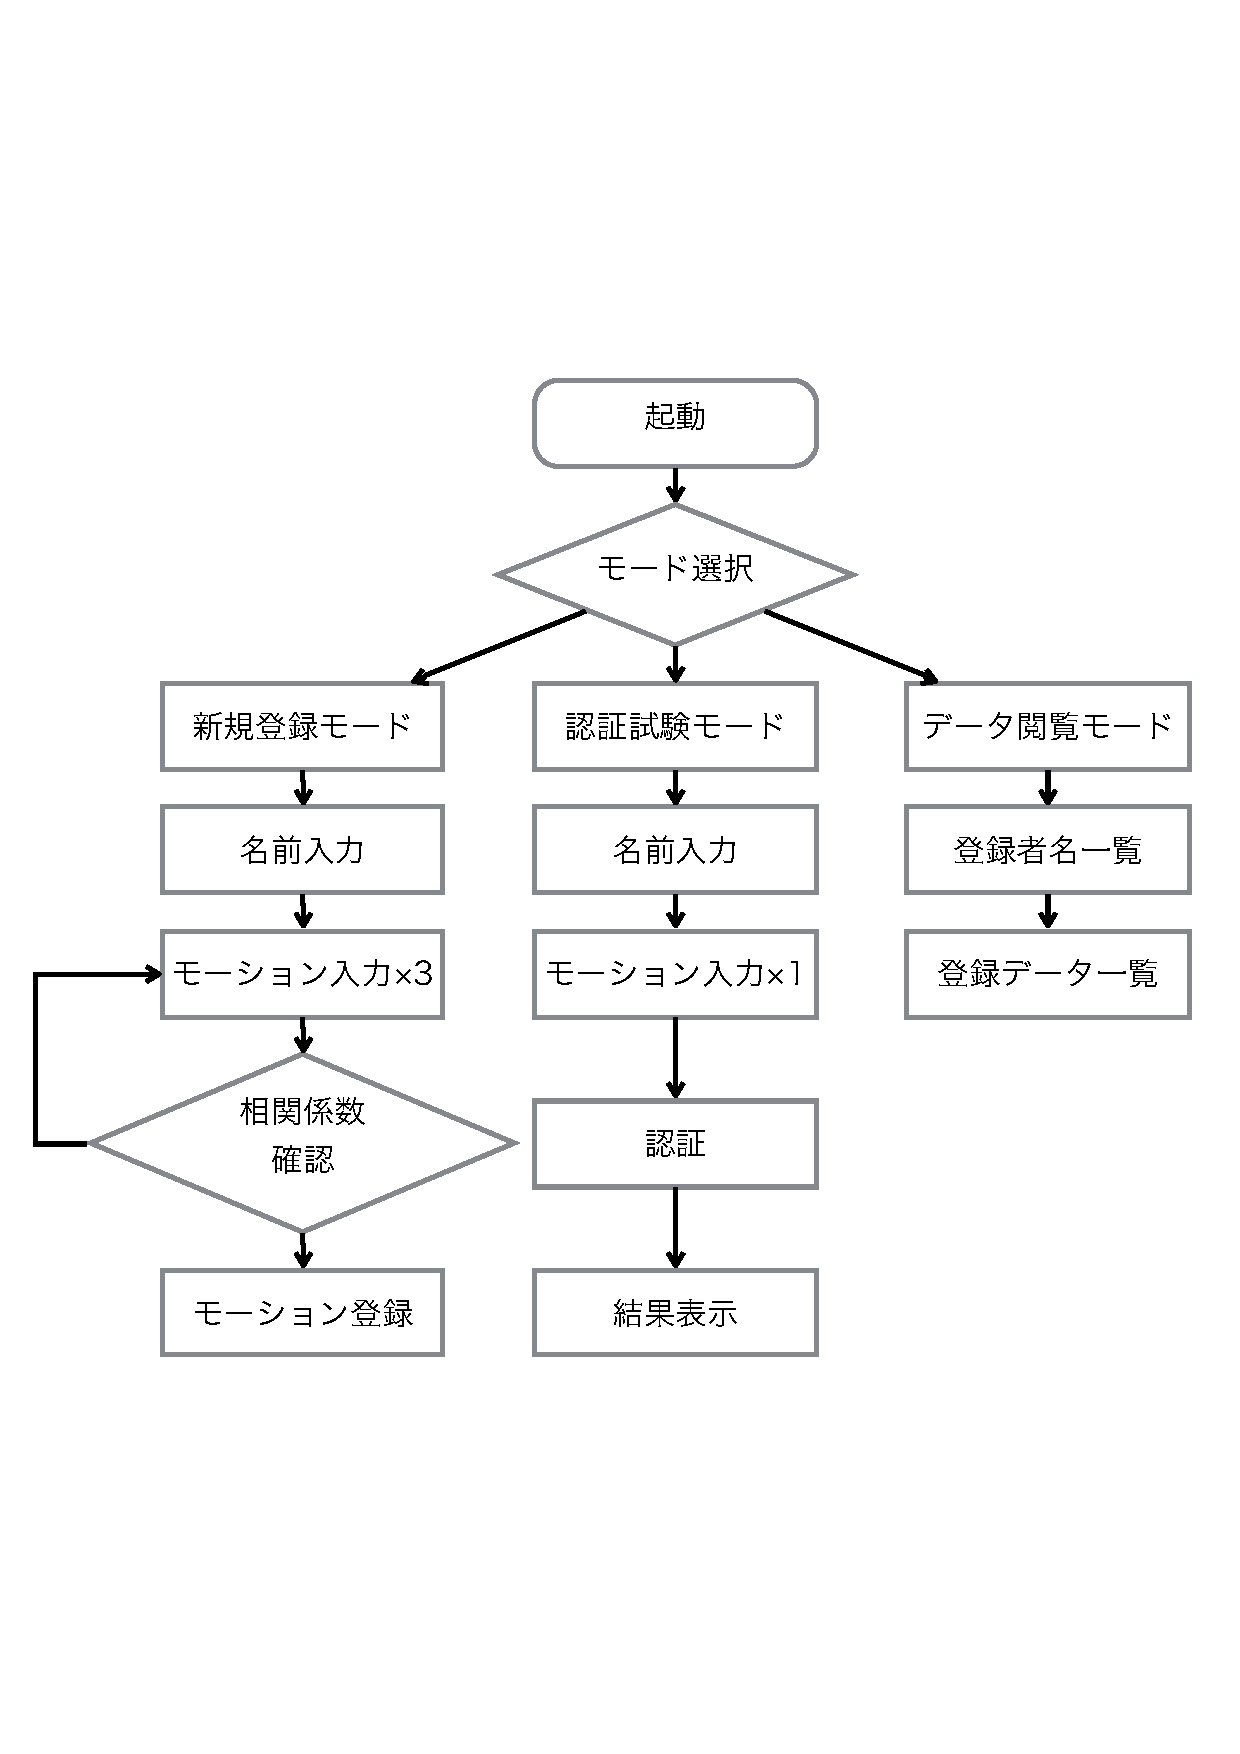
\includegraphics[width=80mm, bb=0 183 590 670]{Flow.pdf}
        \caption{動作フロー図}
        \label{flow}
    \end{center}
\end{wrapfigure}

アプリケーション起動時に表示されるモード選択ダイアログから,まずは新規登録モードを選択する.
このモードでは,ユーザ名を指定して,個人認証を行う際の鍵情報となるモーションデータを登録することができる.
モード選択後,登録したいユーザ名を入力し,モーションの取得を3回行う.
データを取得した後に,その振れ幅を確認する.
あらかじめ設定しておいた増幅器の閾値を元に,取得したデータの振れ幅が1回でも閾値より小さい場合はモーションの動きが小さいと判断し,全てのデータに振れ幅の増幅処理を行う.
次にフーリエ変換を用いたローパスフィルタ処理によって,モーション取得時の手の細かなブレなどから生じうるデータに対する影響を取り除く.
ローパスフィルタ処理が終われば,取得したデータが同一のモーションのものであるかの確認を行う.
同一のモーションであれば,モーション取得時に生じうる時間的なズレを必要に応じて修正する.
同一のモーションでなければ,モーションの取り直しを行う.
時間的なズレを修正する処理が終われば,処理を行った3回分のデータの平均値を算出し,増幅量と共に登録する.

これらの処理を行うことで,先行研究で挙げられていた認証成功率の低さや対応できるモーションに限りがあるという問題に対応している.

認証試験モードでは,あらかじめ新規登録モードにおいてモーションデータの登録を行ったユーザ名を指定し,そのデータと新たに1回入力したモーションデータとの相関係数を算出して個人認証を行う.
この際,新規登録モードにおいてモーションデータと共に登録した増幅量を元に,新たに入力したデータに対しても同様の増幅処理を行う.

データ閲覧モードでは,新規登録モードにおいて登録したユーザ名およびモーションデータをリスト形式で閲覧する事ができる.

\section{実験と考察}
先行研究の課題として挙げられていた,手首を中心とするような比較的小さいモーションに対する認証精度を確認するために,登録および認証の成功率と成功時の平均試行回数を求める実験を行った.
実験の前に任意のモーションで登録と認証を行い,認証に成功できた10名を被験者とした.
実験対象のモーションは5種類とし,手首から先のみを動かすようにしてモーションを入力した.
それぞれの試行回数は3回までとし,これで登録および認証できなかったものは失敗とみなした.
実験結果は以下の表\ref{result}に示すようになった.

% 実験結果
% 試行回数をいずれも平均試行回数(少数あり)にする.
\begin{table}[htb]
    \begin{center}
        \caption{実験結果}
        \label{result}
        \begin{tabular}{|c|r|r||r|r|} \hline
            モーション & 登録成功率 & 平均試行回数 & 認証成功率 & 平均試行回数 \\ \hline \hline
            円を描く & 100\% & 1.1回 & 70\% & 1.7回 \\ \hline
            三拍子を振る & 100\% & 1.0回 & 30\% & 1.6回 \\ \hline
            四拍子を振る & 100\% & 1.0回 & 30\% & 1.0回 \\ \hline
            無限大記号を描く & 100\% & 1.0回 & 80\% & 1.2回 \\ \hline
            四角形を描く & 100\% & 1.0回 & 60\% & 1.5回 \\ \hline
        \end{tabular}
    \end{center}
\end{table}

実験の結果,モーションの登録は被験者のほぼ全員が1回の試行で成功できたが,認証の成功率に関しては高いもので80\%,低いもので30\%という結果となった.
登録においては,データ取得時のズレを修正する処理を施したことによって登録に成功した被験者が見受けられた.

認証成功率の特に低かった三拍子を振るものや四拍子を振るものは,他のものと比較して馴染みの無さがモーションの再現に影響したのではないかと考えている.
また,四拍子を振るものや四角形を描くものは,モーションの取得時間が3秒間である中でこれらを入力しなければならず,再現がしづらかったのではないかと考えている.

\section{今後の課題}
本研究のシステムでは,モーションの登録に関してはほぼ1回の試行で成功できるようになった.
また,認証において再現のしやすいモーションに関しては,手首から先のみを動かして入力する場合でも比較的高い認証成功率を得ることが出来た.
しかし,馴染みの無いモーションや3秒間で入力しづらいモーションに関しては,認証成功率が低くなってしまった.

モーションの取得時間を3秒間に制限することは,モーションの種類を制限してしまうことから本研究の目標とする自由度の高さを制限することになるため,改善が必要であると考える.

また,モーションの登録や認証を他人に覗き見られ,なりすましによる認証が行われた場合にどの程度認証が通ってしまうのかを検証する必要がある.

 % 参考文献
\begin{thebibliography}{9}
    \bibitem{tozawa}兎澤星伸,”三軸加速度センサ及び三軸ジャイロセンサを用いた認証アプリケーションの開発”,2012年度卒業研究.
\end{thebibliography}

\end{document}
